\documentclass[a4paper,10pt]{article}

\usepackage[utf8]{inputenc}
\usepackage{graphicx}
\usepackage[T1]{fontenc}

% Path relative to the main .tex file.
\graphicspath{ {./images/} }

\title{Scalavelli project}

\date{14 Agosto - 15 Settembre 2020}

\author{
Cavalluzzo M.
\and
Giorgietti L.
\and
Pagnini L.
\and
Tentoni D.
}

\begin{document}
    \pagenumbering{gobble} % no numbers.
    \maketitle
    \newpage
    \pagenumbering{arabic} % start counting numbers.

    \begin{abstract}
        Progetto scritto in Scala per giocare al celebre gioco Machivelli sul proprio computer e sfidare altri giocatori.
    \end{abstract}

    \tableofcontents

    \newpage


    \section{Processo di sviluppo}\label{sec:processo-di-sviluppo}

    \subsection{Metodologia}
    Sin da subito abbiamo deciso di adottare una metodologia di sviluppo \textit{Agile-Scrum}, seppur non scegliendo un vero e proprio Scrum Master.
    Chi più e chi meno, a seconda dei vari sprint, ognuno ha avuto l'occasione e il modo di ricoprire tale ruolo.
    In questo modo tutti hanno potuto dare il loro contributo per la riuscita del progetto, coordinando il team con l'aiuto degli strumenti a disposizione.
    In accordo con tale metodologia, il lavoro è stato suddiviso in \textit{Sprint}, della durata media di una settimana e mezzo.
    Allo scadere del tempo si sarebbe dovuti arrivare a sviluppare un numero minimo di funzionalità dell'applicativo.
    I meeting sono stati frequenti all'inizio e ne sono stati svolti alcuni saltuariamente all'interno di ogni sprint.
    Questo perché, alternandosi con un periodo di lavoro autonomo, abbiamo ritenuto necessario e producente confrontarsi anche durante gli sprint su scelte sintattiche e pattern di sviluppo tra tutti i membri del team, in modo da condividere conoscenze ed entusiasmo.

    \subsection{Strumenti adottati}

    \subsubsection{VCS}
    Si è deciso di utilizzare \textit{Git} per effettuare il versioning del codice durante lo sviluppo attraverso la piattaforma \textit{GitHub}.
    L’utilizzo che ne abbiamo fatto è descritto nell'immagine di seguito:
    \begin{center}
        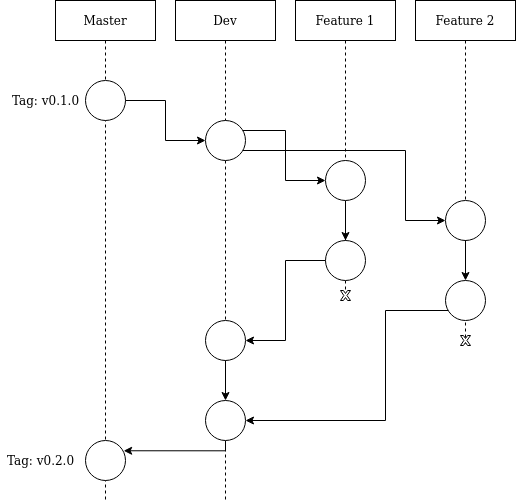
\includegraphics[scale=0.5]{git-workflow-1-1}
    \end{center}

    \subsubsection{Build Automation}
    Si è deciso di usare \textit{SBT}, dato che durante il corso lo si é sempre preferito rispetto al 'cugino' \textit{Gradle} per lo svolgimento degli elaborati, nonostante il fatto che alcuni componenti del gruppo lo utilizzino in ambito aziendale.

    \subsubsection{Continuous Integration}
    Si è deciso di usare \textit{Travis CI}.
    Consisteva nell'unica soluzione freeware che i componenti del gruppo abbiano mai usato, introdotta proprio in questo corso.
    Tuttavia, è stato necessario approfondire l'argomento tramite studio autonomo, dato che ciò che si era appreso a lezione é stato ritenuto insufficiente per la buona riuscita del progetto per come è stato pensato.
    Ad esso é stata adattata l'esecuzione dei test necessari per verificare la correttezza del lavoro svolto e poter poi effettuare dei rilasci senza regressioni.
    Tramite lo stesso servizio é stata effettuata la \textit{Continuous Delivery}, rilasciando dei pacchetti compilati su \textit{Github Releases}.

    \newpage


    \section{Requisiti}\label{sec:requisiti}

    \subsection{Business}\label{subsec:business}
    Il progetto Scalavelli vuole ricreare l’esperienza del celebre gioco di carte Machiavelli (Ramino Machiavellico) in modalità multiplayer, tra giocatori differenti collocati sulla stessa macchina o nella stessa LAN. Ogni giocatore deve potersi identificare con un proprio username e connettersi ad una lobby.
    Essa deve poter contenere da 2 a 6 giocatori.
    Raggiunto il numero necessario di essi si potrà partecipare ad una partita.
    Vi è anche la possibilità di scegliere di giocare specificatamente con i propri amici inserendo il codice identificativo per una partita privata.

    \subsection{Utente}\label{subsec:utente}
    L’utente medio utilizzatore potrà interagire solamente con il client dell’applicazione, tramite le seguenti operazioni in fase di creazione della partita:
    \begin{itemize}
        \item Specificare il proprio username (per potersi registrare nel server) e il numero di giocatori di una partita o inserire il codice di una partita privata che gli è stato inviato o generato da lui stesso;
        \item Inserire o creare una lobby privata;
        \item Connettersi ad una lobby e attendere il raggiungimento del numero di giocatori.
    \end{itemize}

    \subsection{Funzionali}
    \begin{itemize}
        \item Il gioco
        \begin{itemize}
            \item Preparazione del gioco:\newline
            All'inizio della partita devono essere mescolati tra loro due mazzi da 52 carte ognuno (vengono tenuti
            i due Jolly di ogni mazzo).
            Successivamente vengono distribuite 13 carte ad ogni giocatore.
            \item Svolgimento di un turno:\newline
            Il giocatore di turno può compiere le seguenti azioni:
            \begin{itemize}
                \item Giocare una combinazione
                \item Aggiungere carte ad una combinazione già esistente
                \item Prendere carte dal tavolo
                \item Passare il turno
            \end{itemize}
        \end{itemize}
    \end{itemize}

    \subsection{Non Funzionali}
    \begin{itemize}
        \item Scalabilità: Il server deve essere in grado di poter supportare un numero indefinito di utenti.
        Quando
        non sono dentro una partita, i giocatori devono stare in attesa in una lobby per l'arrivo dei giocatori
        necessari per far partire una nuova partita.
    \end{itemize}

    \subsection{Implementativi}

    \newpage


    \section{Design Architetturale}

    \subsection{Model}

    \subsection{View}

    \subsection{Controller}

    \newpage


    \section{Design di Dettaglio}

    \subsection{Organizzazione del codice}
    \begin{center}
        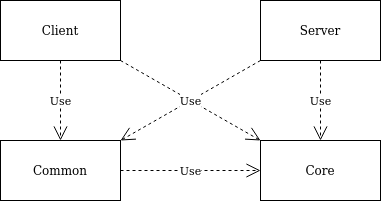
\includegraphics[scale=0.5]{moduli.png}
    \end{center}

    \subsection{Core}

    \subsubsection{Entità}

    \subsubsection{Prolog}

    \subsubsection{Game Interface}

    \subsection{Client}

    \subsubsection{MVC}

    \subsubsection{Lobby}

    \subsubsection{Game}

    \subsection{Server}

    \subsubsection{Lobby}

    \subsubsection{Game}

    \newpage


    \section{Implementazione}

    \subsection{Matteo}

    \subsection{Luca}

    \subsection{Lorenzo}

    \subsection{Daniele}

    \subsubsection{Continuous Integration}
    Io mi sono occupato di configurare opportunamente l'ambiente di CI scelto in modo da poter verificare la
    correttezza di ogni singola build, compilando ad ogni push su ogni branch e pull request.
    Inoltre, viene
    effettuato anche un upload sul sito Codecov.io (che si occupa di mantenere delle statistiche sulla copertura
    dei test sul progetto), del rilascio della Doc e Scaladoc ad ogni rilascio sul branch di sviluppo sull'ambiente
    di Github-Pages in modo da renderlo disponibile per tutti e di effettuare un rilascio dei pacchetti eseguibili
    degli applicativi server e client ad ogni push sul master che sia stata etichettata da un tag.
    Questa parte
    ha richiesto molto lavoro ancora prima di iniziare a sviluppare, ma successivamente tutto il team ne ha tratto
    beneficio.
    Successivamente, in corso d'opera, si è trattato solamente di adattare mano a mano la configurazione
    già esistente alle crescenti esigenze del progetto.
    In primo luogo, il bisogno di stringere i tempi di compilazione
    sull'ambiente remoto, che già all'inizio del progetto, quando quindi era ancora relativamente piccolo, iniziavano
    già a richiedere diversi minuti per ogni singolo passaggio, andandosi a sommare in lunghe compilazioni tra i
    10 e i 15 minuti.
    Successivamente ha richiesto di risolvere qualche problema con la compilazione e l'impacchettamento
    degli eseguibili.

    \subsubsection{Build automation}
    Mi sono occupato inoltre degli script necessari per eseguire agilmente una compilazione di tutto il progetto
    o di parte di esso in base alle esigenze.
    Ho configurato tutto il progetto in modo che fosse logicamente diviso
    in moduli in modo da aumentare l'incapsulamente e l'esposizione ad altre porzioni di progetto di solo le parti
    necessarie.
    Ho inoltre configurato tutti i pacchetti e le librerie aggiuntive da importare nel progetto.

    \subsubsection{Model}
    Assieme a Lorenzo mi sono occupato dello sviluppo delle entità base del progetto e di tutti quegli elementi
    di gioco che riguardavano le regole del gioco e l'iterazione tra di esse.

    \newpage


    \section{Retrospettiva}

    \subsection{Problemi riscontrati}

    \subsection{Sviluppi futuri}

    \newpage

\end{document}
